\documentclass[12pt, a4paper]{article}
\usepackage[style=abnt]{biblatex}
\addbibresource{bibliografia.bib}
\usepackage[utf8]{inputenc} % Pacote para acentuação
\usepackage{csquotes}
\usepackage[portuguese,brazilian]{babel}
\usepackage[lmargin=3cm,tmargin=3cm,rmargin=2cm,bmargin=2cm]{geometry} % Formato que lembra a ABNT
\usepackage[T1]{fontenc} % Ajusta o texto que vem de outras fontes
\usepackage{amsmath,amsthm,amsfonts,amssymb,dsfont,mathtools,blindtext} % Pacotes matemáticos
\usepackage{blindtext} % Texto aleatório
\usepackage{graphicx} % images
\usepackage{indentfirst}
\usepackage{booktabs, multirow} % For borders and merged ranges
\usepackage{soul} % For underlines
\usepackage[table]{xcolor} % For cell colors
\usepackage{changepage,threeparttable} % For wide tables
\usepackage{caption}
\usepackage{float}

\begin{document}

%Capa
\begin{titlepage}
	\begin{center} %centralizar o texto abaixo
		{\begin{figure}[ht]
				\centering
				
\includegraphics[width=9cm]{images/logoUNESP.jpg}
			\end{figure}}
		{\bf \large FEIS – FACULDADE DE ENGENHARIA DE ILHA SOLTEIRA}\\[0.2cm] % o comando \\ "manda" o texto ir para próxima linha
		{\bf \large DEE – DEPARTAMENTO DE ENGENHARIA ELÉTRICA}\\[3.5cm]

		{\large ELE1074 – CIRCUITOS ELÉTRICOS II}\\[4.1cm]

		{\bf \huge 4º Relatório:}\\[0.2cm] % o comando \bf deixa o texto entre chaves em negrito. O comando \huge deixa o texto enorme

		{\bf \huge Filtros passa-faixa e rejeita-faixa}\\[4.1cm]

		{\large Turma: SP2}\\[0.5cm]

		{\begin{tabular}{l c}
			\large\textbf{Aluno(a):}                      & \large\textbf{R.A.:}
			\\
			\Large Enzo Luiz Fernandes                    & \large 181053616     \\
			\Large Maria Luzia Queiroz Barboza dos Santos & \large 181051303
			\\
		\end{tabular}}\\[1cm]

		{\large Professor: Lucas do Carmo Yamaguti}\\[1.1cm]

	\end{center} %término do comando centralizar



	\begin{center}
		{\large Ilha Solteira.}\\[0.2cm]

		{\large 03/02/2021}

	\end{center}
\end{titlepage}
%Sumário
\newpage
\tableofcontents
\thispagestyle{empty}
\pagebreak
\newpage
\section{Objetivos}
Comprovar experimentalmente as teorias matemáticas que descrevem o comportamento de circuitos RLC, como filtro passa-faixa e rejeita-faixa, por meio de simulações e estudo de circuitos.
\pagebreak
\newpage

\section{Resumo}

A experiência consiste no estudo de um circuito RLC paralelo cujo comporta-se como passa-faixa e
como filtro rejeita-faixa, dependendo da tensão de saída análisada (indutor e resistor, respectivamente). Para isso, o sistema foi simulado em um software adequado, e foram analisadas as funções transferência , seu módulo, as frequências de corte, e ressonância. Estes filtros são circuitos capazes de selecionar ou excluir um sinal de sua saída
através dos sinais de entrada. A análise é dada através de gráficos gerados no software, de onde é
possível obter valores e compará-los com resultados de cálculos teóricos. O valor da frequências de corte e de ressonância obtidas
experimentalmente é comparada com o valor obtido através de cálculos, de maneira que o maior erro entre esses seja de
$0,462\%$, o que garante a veracidade dos dados e processos realizados nesta experiência.

\pagebreak
\newpage
\section{Fundamentos Teóricos}
Filtros passa-faixa e rejeita-faixa são circuitos RLC com frequência variável, que conseguem selecionar para sua saída determinados um intervalo de sinais de entrada, atenuando ou acentuando sinais que estejam fora da faixa de passagem. É fato que a resposta de um circuito é dependente de suas impedâncias, logo, uma vez que a impedância é uma função da frequência, tem-se que esta é a principal distinção entre um circuito com frequência constante e outro com frequência variável.

No estudo de resposta em frequência, tem-se que a amplitude e a fase da saída variam somente se a amplitude e a fase da função de transferência também variam, à medida que a frequência é alterada. A função de transferência no circuito de filtro utilizado neste experimento, cujos possuem tensões senoidais como entrada e saída, é dada pela razão entre a tensão de saída e a tensão de entrada.

\begin{figure}[ht]
	\centering
	\caption{Circuito RLC com entrada e saída de tensão, no domínio da frequência .}
	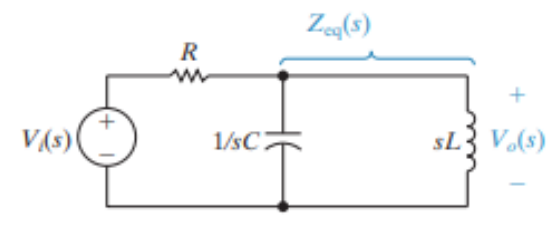
\includegraphics[width=10cm]{imagens/circuitotensao.png}
	\caption*{Fonte:\cite{nilsson2008circuitos}.}
	\label{circuito}
\end{figure}

\begin {equation}
H(s) = \frac{V_o(s)}{V_i(s)}
\label{transferencia}
\end {equation}

O que diferencia um circuito filtro passa-faixa para filtro rejeita-faixa é a análise de seu gráfico de resposta. Os gráficos, mostrados adiante, ilustram a variação da função de transferência com a variação da fonte, onde tem-se os valores de $|H(j\omega)|$ em função da frequência $\omega$ sendo o gráfico da amplitude, e $\theta(j\omega)$ em função da frequência $\omega$ sendo o gráfico de fase.

\subsection{Filtro passa-faixa}

Os filtros passa-faixa são nomeados dessa forma devido ao gráfico de resposta, onde nota-se que o circuito permite apenas a saída de um intervalo entre as frequências de corte $\omega_{c1}$ e $\omega_{c2}$, de modo que atenue as frequências fora desse intervalo, sendo a largura de faixa de passagem, denominada de $\beta$, indicado na equação \ref{beta}, em $rad/s$. A tensão de saída para esse filtro é dada sob os terminais do indutor.

\begin{equation}
	\beta = \omega_{c2} - \omega_{c2} = \frac{1}{RC} \qquad [rad/s]
	\label{beta}
\end{equation}

\begin{figure}[ht]
	\centering
	\caption{Gráfico do filtro passa-faixa ideal.}
	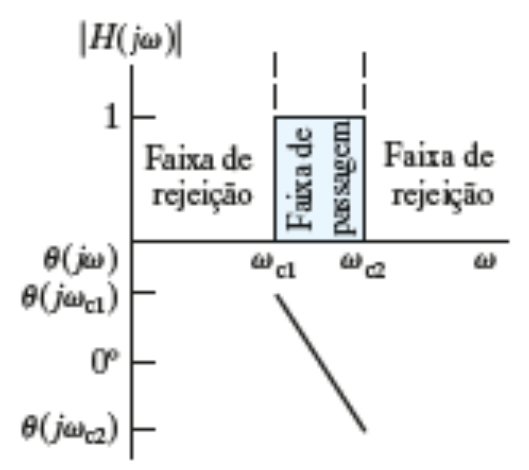
\includegraphics[width=6cm]{imagens/graficoPassaFaixaIdeal.png}
	\caption*{Fonte:\cite{nilsson2008circuitos}.}
	\label{graficoPassaFaixaIdeal}
\end{figure}

\begin{figure}[ht]
	\centering
	\caption{Gráfico do filtro passa-faixa.}
	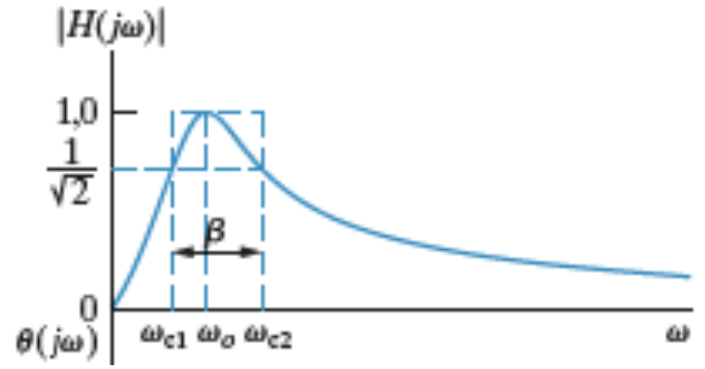
\includegraphics[width=10cm]{imagens/graficoFiltroPassaFaixa.png}
	\caption*{Fonte:\cite{nilsson2008circuitos}.}
\end{figure}

Alguns parâmetros são importantes para a análise dos filtros. A frequência de ressonância, ou natural, $\omega_0$, definida quando quando a função de transferência é um real puro, ou seja, sem parte imaginária; é o valor de frequência que correspondente ao máximo valor do módulo da . Pode ser matematicamente definido pelas equações \refeq{frequência de ressonância 1} ou
\refeq{frequência de ressonância 2}.

\begin {equation}
\omega_0 = \sqrt{\frac{1}{L C}} \qquad [rad/s]
\label{frequência de ressonância 1}
\end {equation}

\begin {equation}
\omega_0 = \sqrt{ {\omega_{c1}}^2 {\omega_{c2}}^2 } \qquad [rad/s]
\label{frequência de ressonância 2}
\end {equation}

O fator de qualidade $Q$, é a medida da largura da faixa de passagem, independente da da localização no eixo das frequência $\omega$.

\begin {equation}
Q = \frac{\omega_0}{\beta}
\label{fator de qualidade}
\end {equation}

Realizando uma análise qualitativa do circuito apresentado na Figura \ref{circuito}, observamos que: Quando $\omega = 0$, o capacitor pode ser considerado um circuito aberto e o indutor um curto-circuito, logo a tensão $V_o(s) = 0 V$. E quando $\omega \rightarrow \infty $, a situação inverte, o capacitor é curto-circuito e o indutor um circuito aberto, então $V_o(s) = 0 V$ dá mesma forma. Já na frequência de ressonância, formulada nas equações \ref{frequência de ressonância 1} e \ref{frequência de ressonância 2}, a impedância combinada tende ao infinito, logo $V_o(s) = V_i(s)$.
Então, nos valores entre as frequências de corte a amplitude da tensão de saída será diferente tensão de entrada, porem não nula.

A função de transferência do circuito $H(s)$ , considerando o indutor como tensão de saída, pode ser obtida primeiramente calculando a impedância equivalente do circuito. Notamos que o sistema é um divisor de tensão, logo:

\begin {equation}
Z_{eq} = \frac{ \frac{L}{C} }{ sL + \frac{1}{sC}}
\end {equation}

Sendo assim, a tensão de saída $V_o (s)$ é dada por:

\begin {equation}
V_o (s) = \frac{Z_{eq}}{Z_{eq} + R} V_i(s) = \frac{\frac{s}{RC}}{ s^2 + \frac{s}{RC} + \frac{1}{LC} } V_i(s) \qquad [V]
\label{V0 passa-faixa}
\end {equation}

Substituindo a equação \refeq{V0 passa-faixa} em \refeq{transferencia}, obtemos:

\begin {equation}
H(s) = \frac{ \frac{s}{RC} }{ s^2 + \frac{s}{RC} + \frac{1}{LC} }
\end {equation}

Se $s=j\omega$, então:

\begin {equation}
H(j \omega) = \frac{\frac{j \omega}{RC}}{ (j \omega)^2 + \frac{j \omega}{RC} + \frac{1}{LC} }
\end {equation}

O módulo de um número complexo é dado pela raiz quadrada da soma dos quadrados do número imaginário e real. Portanto, o módulo dado pela função de transferência é dado por:

\begin {equation}
|H(j \omega)| = \frac{ \frac{\omega}{RC} }{ \sqrt{  ( \frac{ 1 }{LC} - \omega^2 )^2 + (\frac{\omega}{RC})^2} }
\label{moduloFuncaoTransferencia}
\end {equation}

Quando $|H(j \omega)|$ é máximo, temos a que $\omega$ é a frequências natural, onde a primeira parte da soma, dentro da raiz da equação \ref{moduloFuncaoTransferencia} é nula. Isso nos leva a equação \ref{frequência de ressonância 1}.

Já para as frequências de corte $\omega_{c1}$ e $\omega_{c2}$ temos a equação \ref{frequencia de corte}. Como o valor $H_{max} = 1$ para os filtros passivos (passa-altas, passa-baixas, passa-faixa e rejeita-faixa), então ela é constante. Vale ressaltar que a diferença entre filtros ativos e passivos se dá pelos componentes presentes no sistema, se eles forem passivos (capacitores, indutores e resistores) e o filtro também é passivo, já se forem ativos (amplificador
operacional, por exemplo), o filtro é classificado como ativo.

\begin{equation}
	|H(j \omega_{cn})| = \frac{1}{\sqrt{2}} H_{max} = \frac{1}{\sqrt{2}}
	\label{frequencia de corte}
\end{equation}

Substituindo a equação \ref{frequencia de corte} na equação \ref{moduloFuncaoTransferencia}, obtemos o equacionamento de ambas as frequências de corte em $rad/s$:

\begin{equation}
	\omega_{c1} = - \frac{1}{2RC} + \sqrt{ (\frac{1}{2RC})^2 + \frac{1}{LC} } \qquad [rad/s]
	\label{omegaC1}
\end{equation}

\begin{equation}
	\omega_{c2} = + \frac{1}{2RC} + \sqrt{ (\frac{1}{2RC})^2 + \frac{1}{LC} } \qquad [rad/s]
	\label{omegaC2}
\end{equation}

\pagebreak

\subsection{Filtro rejeita-faixa}

Ao contrário do passa faixa, esse filtro permite a passagem de qualquer frequência que não esteja no intervalo entre as frequências de corte $\omega_{c1}$ e $\omega_{c2}$, e atenua valores nesse intervalo, como apresentado na Figura \ref{graficoRejeitaFaixaIdeal}. A tensão de saída para esse filtro é dada sob os terminais do resistor.

\begin{figure}[ht]
	\centering
	\caption{Gráfico do filtro rejeita-faixa ideal.}
	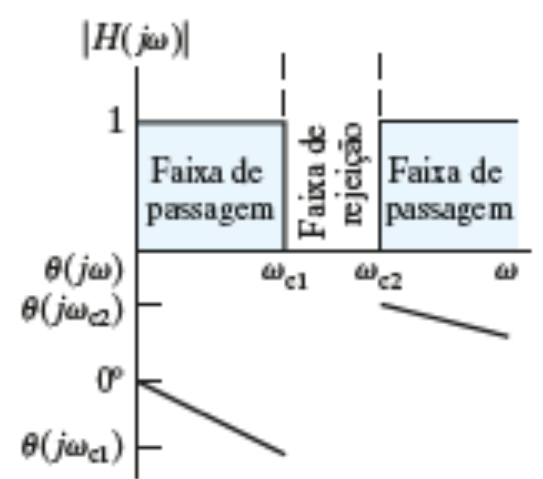
\includegraphics[width=6cm]{imagens/graficoRejeitaFaixaIdeal.png}
	\caption*{Fonte:\cite{nilsson2008circuitos}.}
	\label{graficoRejeitaFaixaIdeal}
\end{figure}

\begin{figure}[ht]
	\centering
	\caption{Gráfico do filtro rejeita-faixa.}
	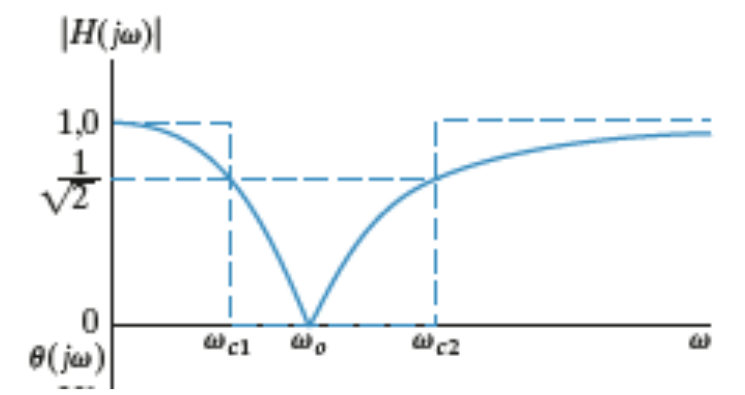
\includegraphics[width=9cm]{imagens/graficoFiltroRejeitaFaixa.png}
	\caption*{Fonte:\cite{nilsson2008circuitos}.}
\end{figure}

A frequência natural $\omega_0$, de um rejeita-faixa é o valor de frequência que correspondente ao mínimo, ou seja, nulo da função de transferência. Os parâmetros, definidos pelas equações \ref{beta}, \ref{frequência de ressonância 1}, \ref{frequência de ressonância 2} e \ref{fator de qualidade}, podem ser aplicadas em ambos os filtros.

Para a analíse qualitativa, vale lembrar que os estados de dos bipolos para $\omega = 0$ e $\omega \rightarrow \infty $ é o mesmo, já que trata-se do mesmo circuito, só mudando o sinal de saída. Quando $\omega = 0$ ou $\omega \rightarrow \infty $, $V_o(s) = V_i(s)$.

Para encontrarmos a função de transferência do filtro rejeita-faixa primeiro devemos observar que, pela analíse de malha obtemos as seguintes relações:

\begin{equation}
	V_i(s) = I (\frac{sL}{s^2LC+1}+R) \qquad [V]
\end{equation}

\begin{equation}
	V_o(s) = IR \qquad [V]
\end{equation}

A partir disso, seguimos os mesmos passos discutidos no tópico anterior, então a função de transferência será:

\begin{equation}
	H(s) = \frac{s^2 + \frac{1}{LC}}{s^2 + \frac{s}{RC} + \frac{1}{LC}}
	\label{funcao tranferenci rejeita-faixa}
\end{equation}

Como $s=j\omega$:

\begin{equation}
	H(j\omega) = \frac{-\omega^2 + \frac{1}{LC}}{-\omega^2 + \frac{j\omega}{RC} + \frac{1}{LC}}
	\label{funcao tranferenci rejeita-faixa jw}
\end{equation}

Calculando o módulo da função:

\begin {equation}
|H(j \omega)| = \frac{ (\frac{1}{LC})^2 - \omega^2 }{ \sqrt{  ( \frac{ 1 }{LC} - \omega^2 )^2 + (\frac{\omega}{RC})^2} }
\label{moduloFuncaoTransferencia2}
\end {equation}

Por fim, ao analisarmos a equação \ref{moduloFuncaoTransferencia2}, da mesma forma do tópico anterior, obteremos as mesmas equações \refeq{omegaC1} e \refeq{omegaC2}.

\pagebreak

\newpage
\section{Procedimento Experimental}

\subsection{Materiais Utilizados}

\subsubsection{Materiais de Laboratório}
Os materiais utilizados em bancada foram:

\begin{itemize}
	\item Conectores de cobre;
	\item Resistor de $1 k\Omega$;
	\item Capacitor de $1 \mu F$;
	\item indutor de $10 mH$
	\item Módulo PU-2222;
	\item Protoboard;
	\item Gerador de função;
	\item Conectores “Banana-jacaré”;
	\item Osciloscópio digital;

\end{itemize}

\subsubsection{Softwares de Simulação}
O software utilizado para simulação do circuito foi o Multisim Live \cite{multisim}, um software de simulação de circuitos gratuito e eficiente perante os objetivos do experimento.

\subsection{Metodologia}
À priori, o circuito foi analisado diante dos seguintes aspectos: Função de transferência, o módulo da função de transferência, para $\omega=0$, $\omega\rightarrow\infty$ e $\omega=\omega_n$, tanto considerando a tensão de saída como a tensão sobre o resistor (filtro rejeita-faixa), quanto a tensão sobre o paralelo LC (filtro passa-faixa).

É importante ressaltar que neste experimento, o filtro passa-faixa e filtro rejeita-faixa são analisados no mesmo circuito, portanto, o mesmo deve ser montado (vide Figura \ref{circuitoSimulado}, e assim é possível analisar ambos os comportamentos simultaneamente. Veremos com mais detalhes a seguir.

É necessário que, além do circuito apresentado no roteiro (Figura \ref{circuitoRoteiro}), sejam incluídos o terra e os voltímetros. Com os voltímetros localizados nestes pontos, é possível analisar a tensão nas extremidades do resistor com PR2 e no paralelo entre o indutor e o capacitor, com PR1. Com isso, a frequência deve ser alterada manualmente perante os valores de $\omega_{C1}$, $\omega_{C2}$ e $\omega_0$ calculados teóricamente, com o objetivo de observar e analisar as respostas gráficas do circuito. Além das frequências em questão, as respostas também devem ser analisadas para os valores presentes na tabela disponibilizada no roteiro, de modo que as lacunas possam ser preenchidas.

\begin{figure}[H]
	\centering
	\caption{Diagrama do Circuito RLC.}
	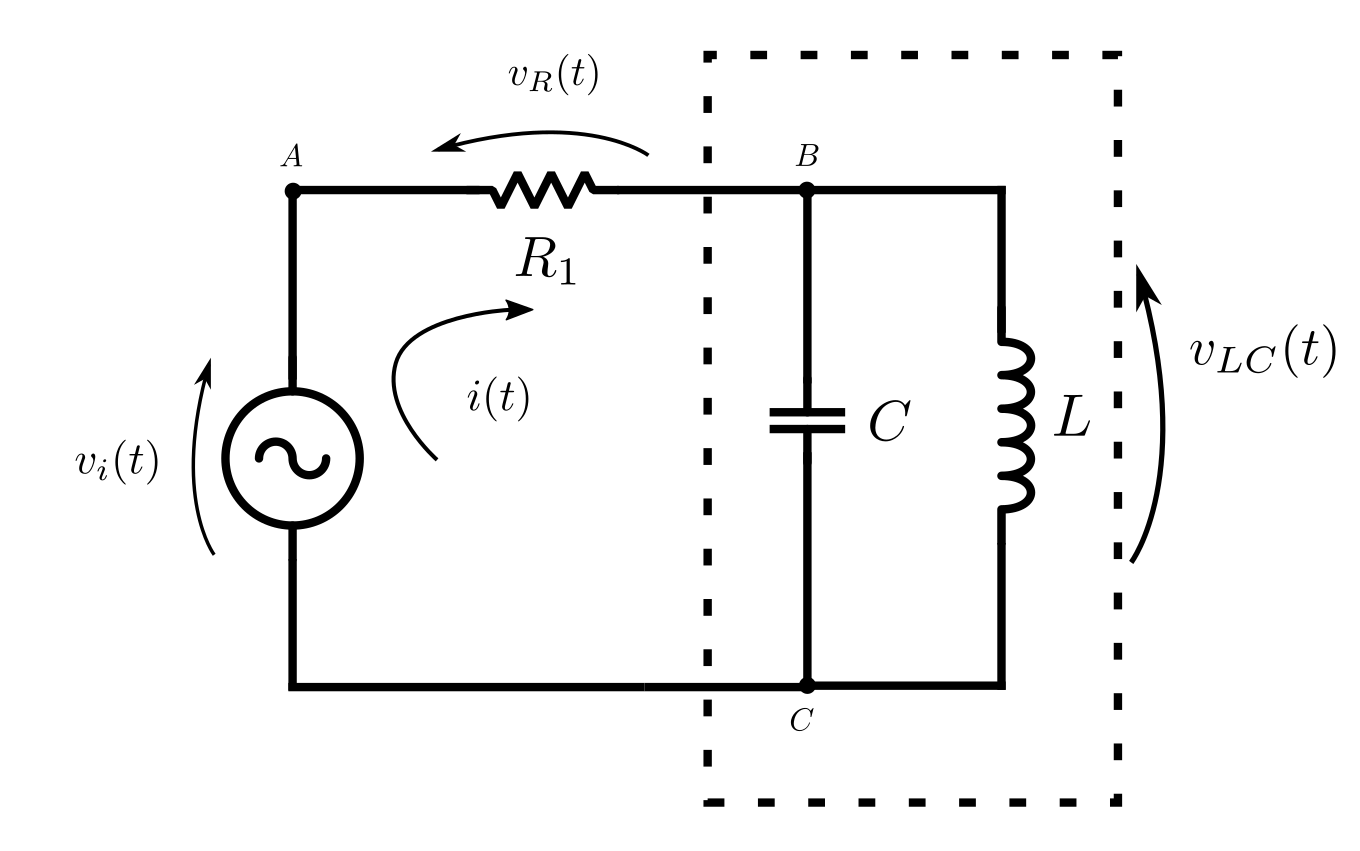
\includegraphics[width=15cm]{imagens/circuitoRoteiro.png}
	\caption*{Fonte: \cite{roteiro4}.}
	\label{circuitoRoteiro}
\end{figure}

\pagebreak
\newpage
\section{Resultados e Discussão}

Como resultado da simulação do circuito da Figura \ref{circuitoSimulado}, obtivemos os seguintes resultados:

\begin{figure}[H]
	\centering
	\caption{Circuito RLC paralelo simulado no Multisim Live.}
	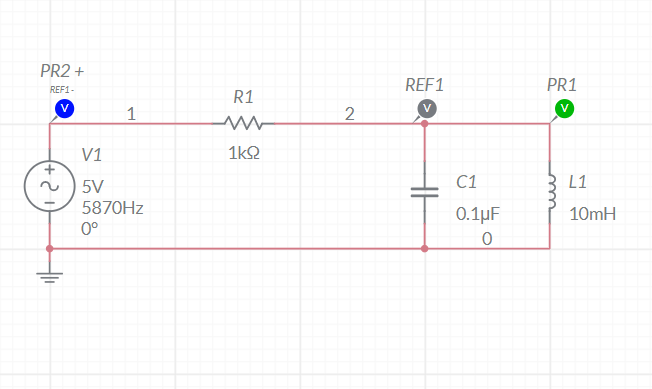
\includegraphics[width=15cm]{images/circuitoSimulado.png}
	\caption*{Fonte: Elaborado pelos autores.}
	\label{circuitoSimulado}
\end{figure}

\subsection{Filtro passa-faixa}
O módulo da função de transferência do circuito como filtro passa-faixa foi calculado para os valores de $\omega=0$, $\omega=\omega_n$ e $\omega\rightarrow\infty$, utilizando a equação \refeq{moduloFuncaoTransferencia}:
\begin{equation}
	\omega=0 \Rightarrow  |H(j\omega)|= 0
\end{equation}
\begin{equation}
	\omega=\omega_n \Rightarrow |H(j\omega)|= 1
\end{equation}
\begin{equation}
	\omega\rightarrow\infty \Rightarrow |H(j\omega)|= 0
\end{equation}

As frequências de corte $\omega_{c1}$ e $\omega_{c2}$, além da frequência de ressonância $\omega_0$ foram calculadas e convertidas para $Hz$, os resultados são apresentados a seguir, utilizando as equações \refeq{omegaC1}, \refeq{omegaC2} e \refeq{frequência de ressonância 2}:

\begin{equation}
	\omega_{C1}= -\frac{1}{2RC}+\sqrt{(\frac{1}{2RC})^2+\frac{1}{LC}}= 4302 Hz
\end{equation}
\begin{equation}
	\omega_{C2}=\frac{1}{2RC}+\sqrt{(\frac{1}{2RC})^2+\frac{1}{LC}}= 5894 Hz
\end{equation}
\begin{equation}
	\omega_0=\sqrt{\frac{1}{LC}}= 5036 Hz
\end{equation}

A conversão para $Hz$ foi dada devido a necessidade de utilizar as frequências dentro do simulador, cujo aceita apenas nesta unidade de medida.

\subsection{Filtro rejeita-faixa}
Quando o circuito se comporta como um filtro rejeita-faixa, sua função de transferência é diferente, pois agora o sinal de saída é dado pela tensão sob o resistor. Sendo assim, o módulo desta função para os diferentes valores de $\omega$ são calculados novamente, dessa vez utilizando a equação \refeq{moduloFuncaoTransferencia2}.
\begin{equation}
	\omega=0 \Rightarrow |H(j\omega)|= 1
\end{equation}
\begin{equation}
	\omega=\omega_n \Rightarrow |H(j\omega)|= 0
\end{equation}
\begin{equation}
	\omega\rightarrow\infty \Rightarrow |H(j\omega)|= 1
\end{equation}

As frequências de corte também foram calculadas para os novos valores, e também convertidas para Hz. A frequência de ressonância é a mesma para ambos os comportamentos do circuito, logo são utilizadas as equações \refeq{omegaC1}, \refeq{omegaC2} e \refeq{frequência de ressonância 2}:

\begin{equation}
	\omega_{C1}=\omega_0[-\frac{1}{2Q}+\sqrt{1+(\frac{1}{2Q})^2}]= 4299 Hz
\end{equation}
\begin{equation}
	\omega_{C2}=\omega_0[\frac{1}{2Q}+\sqrt{1+(\frac{1}{2Q})^2}]= 5891 Hz
\end{equation}
Sendo o fator de qualidade $Q= 3,162$, para ambos os filtros, de acordo com a equação \refeq{fator de qualidade}.

Um ponto importante a ser observado é que as frequências de corte do filtro rejeita-faixa são muito próximas dos valores calculados para o filtro passa-faixa, o que possibilita concluir que por ser o mesmo circuito, a faixa de frequência é a mesma.

\subsection{Simulação}

Com o circuito montado no software, a frequência dos sinais foi definida, à priori, como a frequência de corte $\omega_{C1}$ e ajustada até que o gráfico gerasse a resposta esperada:

Em torno deste valor de frequência inicia-se a faixa de frequência do circuito. Observa-se que a tensão no resistor e no conjunto LC são aproximadamente iguais, e espera-se que o comportamento seja o mesmo em torno da frequência $\omega_{C2}$. Simulando o circuito nestas condições:

\begin{figure}[H]
	\centering
	\caption{Resposta do circuito para a frequência $\omega_{c1}$.}
	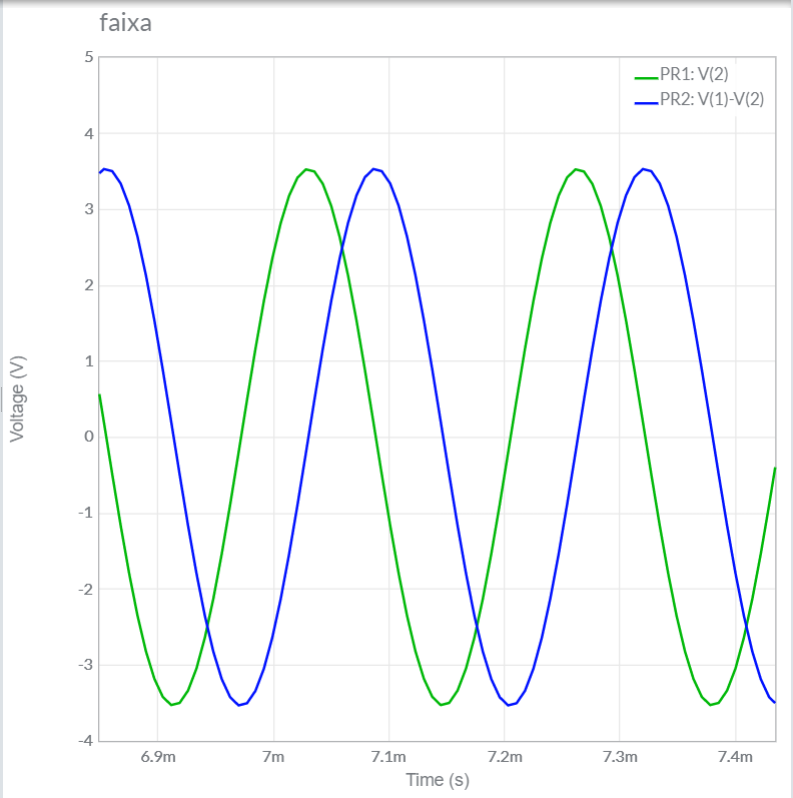
\includegraphics[width=10cm]{images/f_c1.png}
	\caption*{Fonte: Elaborado pelos autores.}
	\label{c1}
\end{figure}

\begin{figure}[H]
	\centering
	\caption{Resposta do circuito para a frequência $\omega_{c2}$.}
	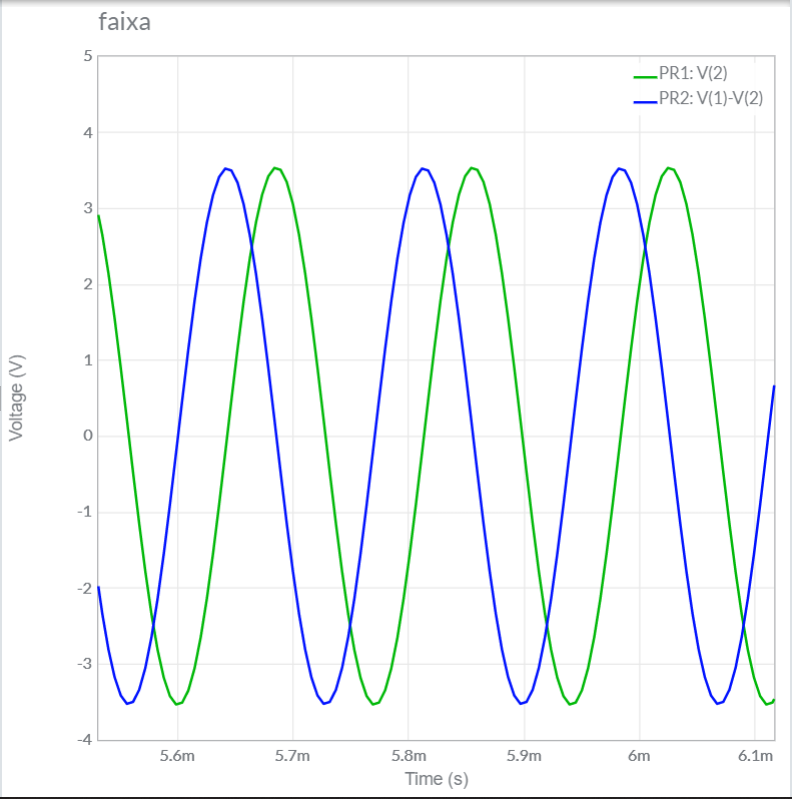
\includegraphics[width=10cm]{images/f_c2.png}
	\caption*{Fonte: Elaborado pelos autores.}
	\label{c2}
\end{figure}

O comportamento esperado é correto e novamente os valores de tensão no resistor e no conjunto LC são aproximadamente iguais, estes são apresentados na Tabela \ref{tabela} e devidamente comparados, tal como as respostas para a frequência de ressonância $\omega_0$, analisadas no gráfico da figura abaixo.

\begin{figure}[H]
	\centering
	\caption{Resposta do circuito para a frequência de ressonância $\omega_0$.}
	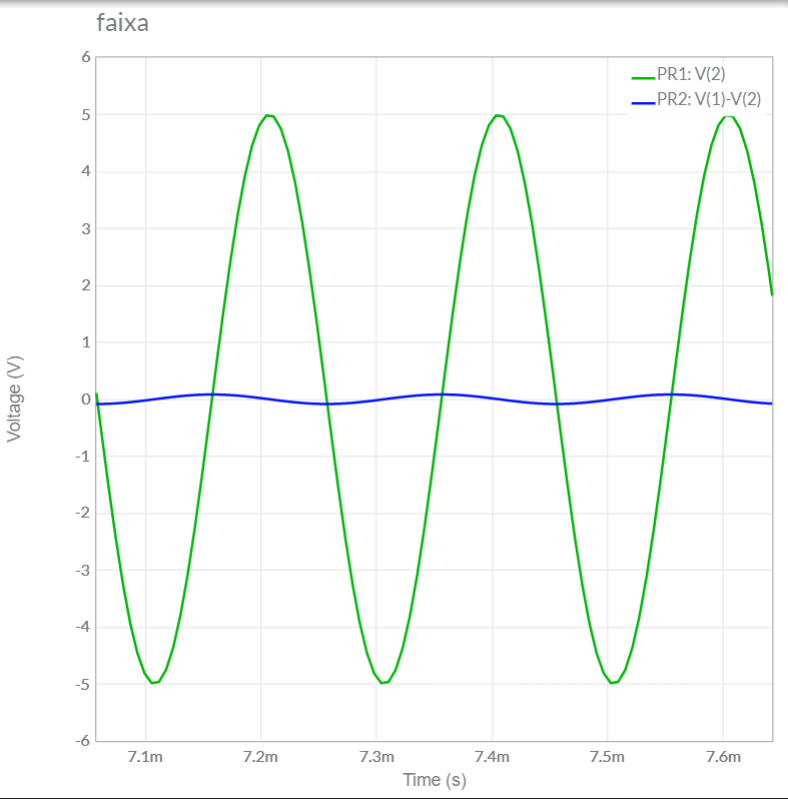
\includegraphics[width=10cm]{images/f_ressonancia.png}
	\caption*{Fonte: Elaborado pelos autores.}
	\label{ressonancia}
\end{figure}

Com o circuito respondendo à $\omega_0$, obtém-se o valor mínimo da tensão sobre o resistor, e o valor máximo da tensão sobre LC.

Para preencher as lacunas da tabela apresentada no roteiro, a operação foi repetida para mais alguns valores de frequência, e todas as respostas foram registradas, além do módulo da função de transferência para os dois diferentes filtros.

\begin{table}[H]
	\caption{Respostas do circuito RLC paralelo.}

	\begin{center}
		\resizebox{\textwidth}{!}{%
			\begin{tabular}{llllll}
				\hline
				\textbf{Frequência ($Hz$)} & \textbf{$v_i(t)$ ($V_{pp}$)} & \textbf{$v_R(t)$ ($V_{pp}$)} & \textbf{$v_C(t)$ ($V_{pp}$)} & \textbf{ $|H(j\omega)|$ (passa-faixa)} & \textbf{ $|H(j\omega)|$ (rejeita-faixa)} \\
				\hline
				785                        & 5                            & 4,9759                       & 0,0025                       & 0,0505                                 & 0,9987                                   \\
				2285                       & 5                            & 4,9184                       & 0,0089                       & 0,1780                                 & 0,9840                                   \\
				3285                       & 5                            & 4,7006                       & 1,7039                       & 0,3384                                 & 0,9410                                   \\
				3785                       & 5                            & 4,3722                       & 2,4216                       & 0,4802                                 & 0,8772                                   \\
				4285                       & 5                            & 3,5319                       & 3,5275                       & 0,6994                                 & 0,7147                                   \\
				4485                       & 5                            & 2,8935                       & 4,0748                       & 0,8075                                 & 0,5899                                   \\
				4785                       & 5                            & 1,4325                       & 4,7873                       & 0,9525                                 & 0,3044                                   \\
				5030                       & 5                            & 0,0064                       & 4,9843                       & 1,0000                                 & 0,0037                                   \\
				5370                       & 5                            & 1,8734                       & 4,6268                       & 0,9252                                 & -0,3796                                  \\
				5570                       & 5                            & 2,7280                       & 4,2488                       & 0,8414                                 & -0,5405                                  \\
				5870                       & 5                            & 3,5244                       & 3,5333                       & 0,7153                                 & -0,6988                                  \\
				6370                       & 5                            & 4,1159                       & 3,1502                       & 0,5537                                 & -0,8327                                  \\
				6870                       & 5                            & 4,6373                       & 2,0396                       & 0,4472                                 & -0,8944                                  \\
				7870                       & 5                            & 4,7514                       & 1,6703                       & 0,3237                                 & -0,9461                                  \\
				9370                       & 5                            & 4,8380                       & 1,2132                       & 0,2322                                 & -0,9727                                  \\
				\hline
			\end{tabular}}

	\end{center}
	\caption*{Fonte: Elaborado pelos autores.}
	\label{tabela}
\end{table}

A largura de banda do circuito é calculada experimentalmente e teoricamente (vide equação \refeq{beta}), tal como o erro percentual entre estes valores e entre as frequências também fora calculado.
\begin{equation}
	\beta_{t} = 10^4 Hz
\end{equation}
\begin{equation}
	\beta_{e} = 9,9538.10^3 Hz
\end{equation}
\begin{equation}
	\%E = 0,462\%
\end{equation}
Frequência de corte inicial:
\begin{equation}
	\%E = 0,395\%
\end{equation}
Frequência de corte final:
\begin{equation}
	\%E = 0,407\%
\end{equation}
Frequência de ressonância:
\begin{equation}
	\%E = 0,119\%
\end{equation}

\pagebreak
\newpage
\section{Conclusão}

Através deste experimento foi possível verificar de forma prática as respostas de um circuito RLC paralelo para determinadas frequências, comportando-se como um filtro passa-faixa ou um filtro rejeita-faixa. Os valores de frequência teóricamente calculados foram comparados com os valores obtidos experimentalmente, e o erro máximo foi de $0,462\%$, sendo assim, um erro desprezível diante das aproximações teóricas e provenientes dos arrendondamentos do software e da análise gráfica. 

\pagebreak
\newpage
\printbibliography[heading=bibintoc, title={Referências}]
\pagebreak

\end{document}